%!TEX root = ../../../../report.tex

\subsection{The electric actuators} % (fold)
\label{sub:electric_actuators}
In chapter \ref{cha:mathematical_model}, the necessary characteristics of the actuators have been calculated.
In this section, the resulting theoretical requirements are used to select the final motor $+$ gearbox combination utilized.
All the documentation regarding the control of the actuators software-wise is to be found in section \ref{sec:software}.

\subsubsection{Flat BLDC Maxon motors} % (fold)
\label{ssub:the_bldc_motors}
It must be mentioned at this point that the actuators and their interface were assumed at the beginning of the project to be a very hard constraint in the design from an economic point of view. 
This means that the conception of the robot structure has been influenced by this criteria towards the adaption of the final prototype characteristics (such as final size or mass) to the application range of the available motors at our disposal.
This fact has converted the design in an iterative process of optimization whose final result is a robot that matches the available actuators and not the other way around, as it should be in theory.
In the view of the this, the brushless DC motor $+$ gearbox present in the Locokit robot construction kit, introduced in \cite{locokit} are used in the Rubi prototype.

The flat motors model is 339260 from Maxon motor, whose datasheet can be found in \cite{maxon_motor}, and the planetary gearhead is the number 143976 in datasheet \cite{maxon_gear}.
The electromechanical constants of the motors, together with its nominal supply values or the output power and torque of both the motor and the gearbox can be found in these documents. 
However, the electronics of the motors are designed to constantly overdrive them at $24V$, which has been taken into account when calculating their output.
Furthermore, each motor counts three hall effect sensors able to provide accurate relative position measurements.

\todo{Add here motor curves from experiments}

% subsubsection the_bldc_motors (end)


\subsubsection{BLDC motor boards} % (fold)
\label{ssub:bldc_motor_boards}
Each BLDC motor in the Locokit comes with a motor board able to control it, designed for 24V and 48W.
They consist of a 48MHz ARM7 processor for time critical control and motor commutation, as stated in \cite{locokit-electronics}, together with 4 general purpose I/O inputs for local sensor interface.
Furthermore, they have two available 8-pin interfaces for the motors, one of them with a standard flex connector used in most of Maxon flat motors.

% subsubsection bldc_motor_boards (end)

\subsubsection{Extension PCBs} % (fold)
\label{ssub:extension_pcbs}
Following the idea of reducing weight and inertias in the structure as explained in chapter \ref{cha:analysis}, it was decided to place all the electronics off-board.
In order to extend the existing motor flex interfaces, a simple extension PCB was manufactured for each device.
The boards have been designed with Eagle following the requirements of current when sizing the width of the paths given by the supplier.
The design lacks of vias which reduces the complexity and facilitates the manufacturing.
The board for the left leg, whose schematic can be seen in \ref{fig:pcb1} \footnote{For the right leg the schematic has been mirrored}, contains a flex connector, like the one originally found on the motor boards, mapped to an 8-pin Molex connector where the wiring to the BLDC board is connected.

\begin{figure}[ht]
	\centering
	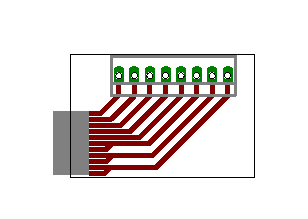
\includegraphics[width=0.5\textwidth]{figures/expansion_board.pdf}
	\caption{Left leg extension PCB schematic}
	\label{fig:pcb1}
\end{figure}

% subsubsection extension_pcbs (end)


% subsection electric_actuators (end)